\chapter{Interface de Administração}

O Aero possui uma interface administrativa com login em \verb|/area/restrita|. 
Para se autenticar,
o usuário deve digitar seu nome de usuário, senha e código TOTP (a autenticação
de dois fatores por tempo). A senha é armazenada no banco com hash e salt usando 
o padrão bcrypt. Para o TOTP é utilizada a biblioteca pyOTP. 

\begin{figure}[H]
    \begin{center}
    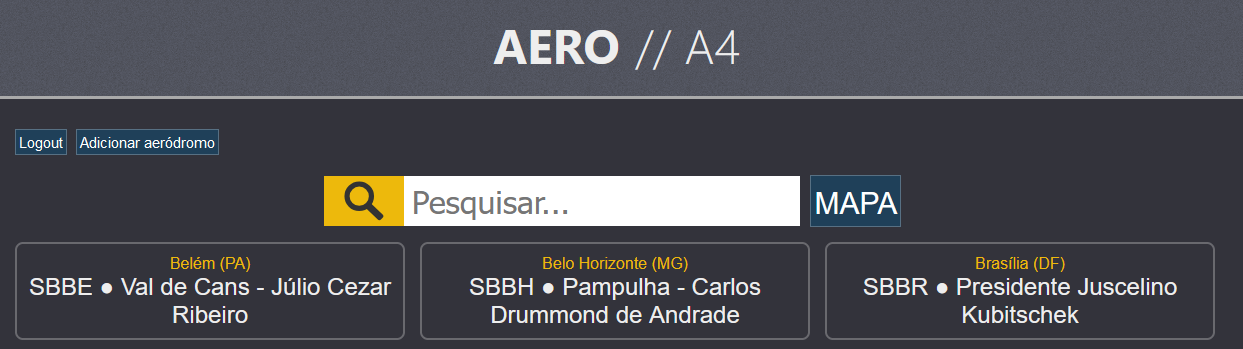
\includegraphics[width=\linewidth]{img/area-restrita-root.png}
    \caption{Tela inicial da área logada}
    \label{fig:max-priv-sys}
    \end{center}
\end{figure}

Para criar e alterar as contas usa-se o script "monitor.py" executado dentro
de um SSH.
O script monitor.py permite fazer diversas operações de máximo privilégio 
incluindo criar, alterar senha e TOTP e apagar usuários. Forçar a atualização de
METARs e TAFs também é possível. Tais tarefas não são 
feitas com frequência. O que é feito com maior frequência é a adição de aeroportos 
e alteração deles.

\begin{figure}[H]
    \begin{center}
    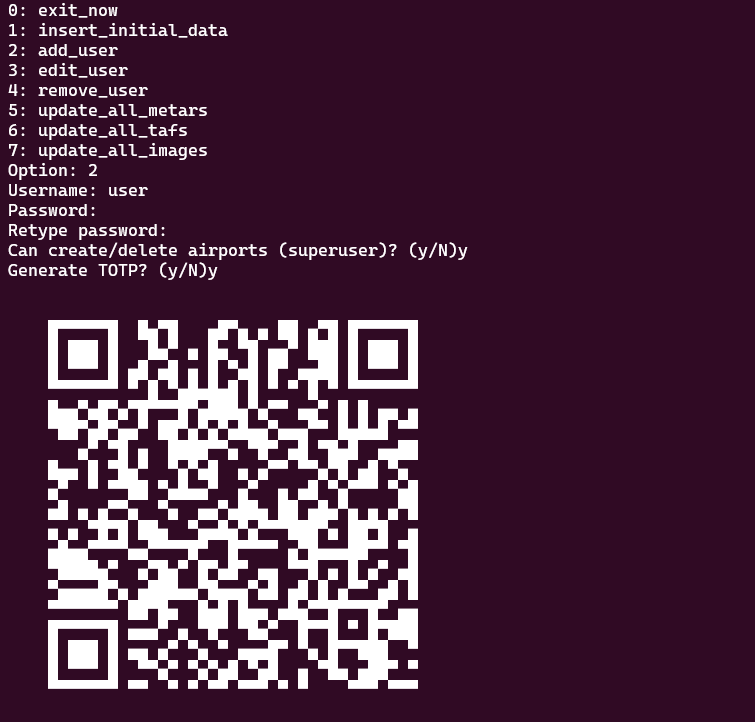
\includegraphics[width=0.8\linewidth]{img/create-user-script.png}
    \caption{monitor.py}
    \label{fig:max-priv-sys}
    \end{center}
\end{figure}

Um usuário com o \verb|isSuper| em verdadeiro pode adicionar e remover aeródromos 
bem como editar e remover qualquer aeródromo. Um usuário normal pode apenas alterar 
aeródromos com ICAO fazendo parte da lista autorizada para ele no momento da criação
de sua conta.

O login é mantido via cookie assinado com padrão JWT de forma que não é custoso 
(não envolve acesso ao banco) verificar se está logado. É usada a biblioteca padrão 
do \textit{fastAPI} já que ela assina os cookies automaticamente.
Ao estar logado, na tela inicial, dois botões são mostrados, o de logout e o de adicionar 
aeródromo. Caso o usuário não seja super o segundo botão não aparece e, obviamente, 
a rota GET e POST de adicionar aeródromo retorna um erro.


Ao entrar em um aerodromo, caso tenha permissão de altera-lo, a seguinte tela
é mostrada.

\begin{figure}[H]
    \begin{center}
    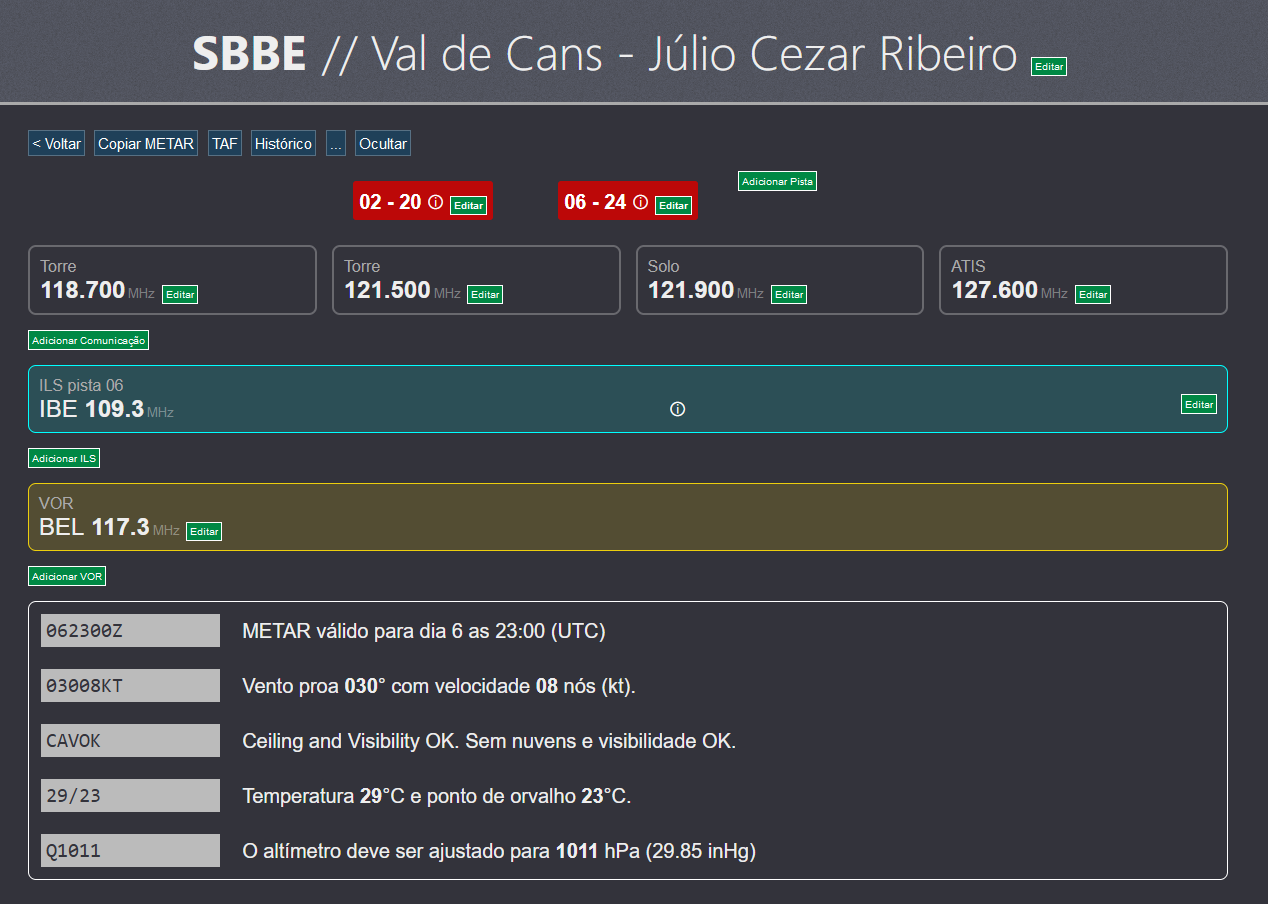
\includegraphics[width=\linewidth]{img/admin-root.png}
    \caption{Tela de aeródromo da área logada}
    \label{fig:max-priv-sys}
    \end{center}
\end{figure}

Pressionando nos botões verdes, é possível criar e alterar qualquer dado do
aeroporto. Dentro da edição de um aeródromo é possível, apagá-lo.

\section {Adicionar/editar aeródromo}
Caso tenha permissão a rota \verb|/area/restrita/add| permite adicionar um aeródromo. 

\begin{figure}[H]
    \begin{center}
    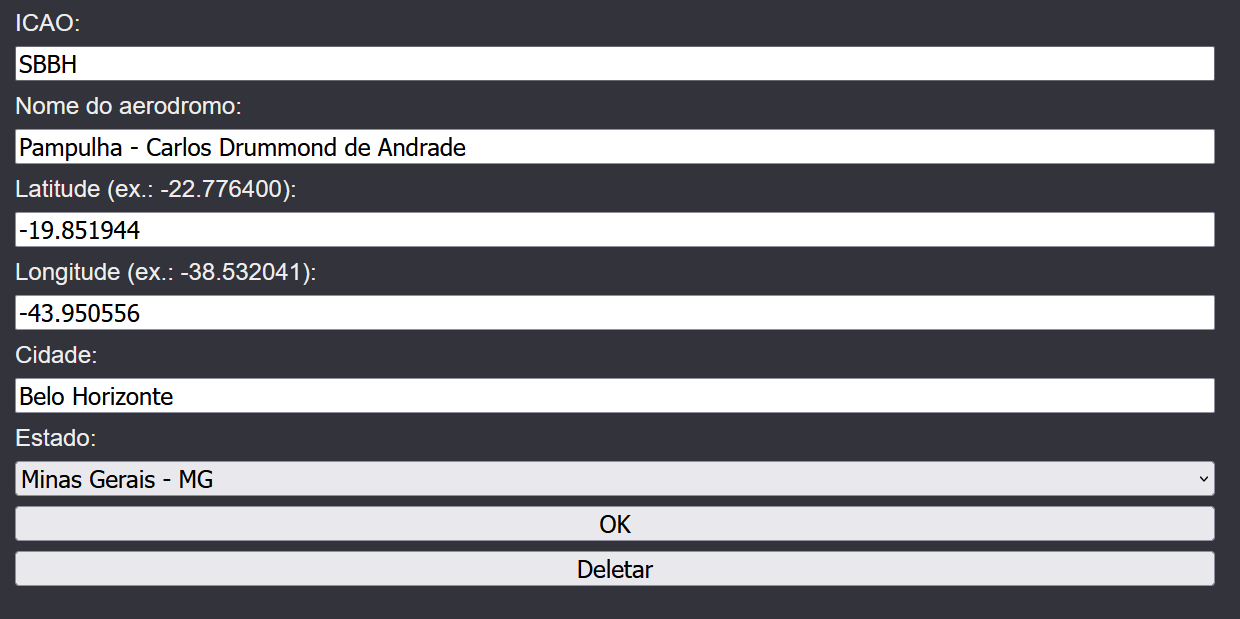
\includegraphics[width=\linewidth]{img/area-restrita-aerodrome.png}
    \caption{Tela de adicionar / editar um aeródromo}
    \label{fig:max-priv-sys}
    \end{center}
\end{figure}

Obviamente o botão de apagar aparece apenas na tela de edição.

Todos os campos possuem algum tipo de validação tanto via HTML quanto via servidor. 
Caso o HTML fosse alterado via developer tools, mesmo que rotas de administração 
são acessíveis apenas por usuários autorizados, ainda assim não seria possível 
para um bad actor adicionar no banco um record inválido.

As validações para esta rota são:
\begin{longtable}{|p{3cm}|p{4.2cm}|p{4.2cm}|}
    \caption{Rotas: /area/restrita/<icao>/edit e /area/restrita/add} \\
    \hline
    \textbf{Campo} & \textbf{Frontend} & \textbf{Backend} \\ \hline
    \endfirsthead
    \multicolumn{3}{c}%
    {{\tablename\ \thetable{} -- Continuação da página anterior}} \\
    \hline
    \textbf{Campo} & \textbf{Frontend} & \textbf{Backend} \\ \hline
    \endhead
    \hline \multicolumn{3}{|r|}{{Continua na próxima página}} \\ \hline
    \endfoot
    \hline
    \endlastfoot
        ICAO
        & Regex: \verb|[A-Z]{4}|
        & Regex: \verb|[A-Z]{4}|
        \\ \hline
        Nome do aerodromo
        & Type: Text
        & String
        \\ \hline
        Latitude
        & Regex: \verb|-?[0-9]*\.[0-9]{6}|
        & Regex: \verb|-?[0-9]*\.[0-9]{6}|
        \\ \hline
        Longitude
        & Regex: \verb|-?[0-9]*\.[0-9]{6}|
        & Regex: \verb|-?[0-9]*\.[0-9]{6}|
        \\ \hline
        Cidade
        & Type: Text
        & Verificar se a cidade existe no estado via API do IBGE
        \\ \hline 
        Estado
        & Menu dropdown (select/option)
        & Existe na lista de estados do Brasil
        \\ \hline 
\end{longtable}

\section {Adicionar/editar pista}

\begin{figure}[H]
    \begin{center}
    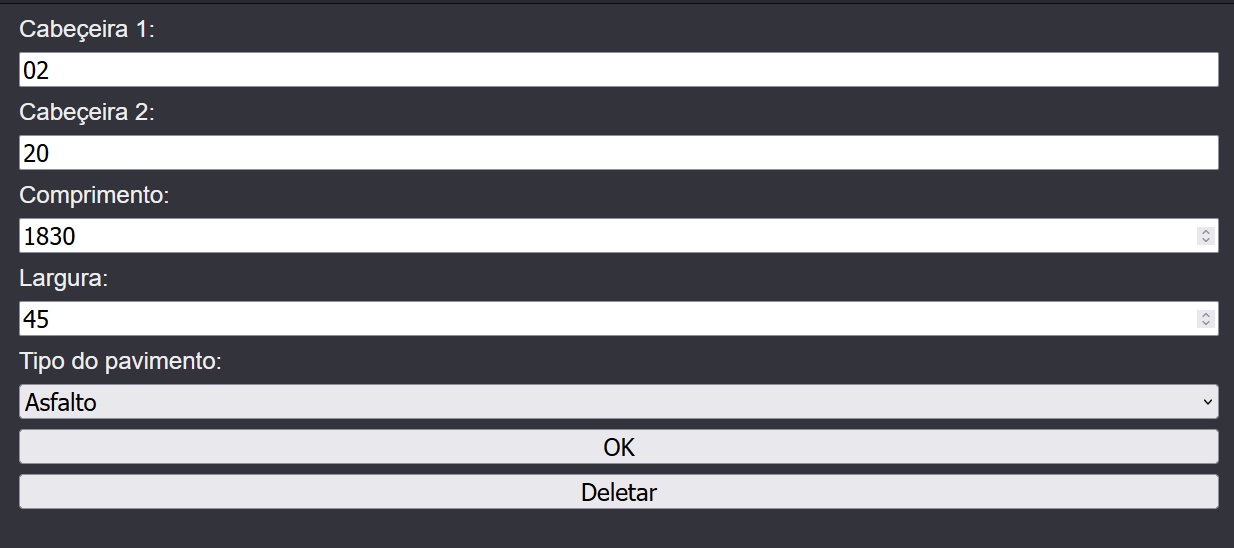
\includegraphics[width=0.7\linewidth]{img/admin-edit-runway.png}
    \caption{Tela de adicionar / editar uma pista}
    \label{fig:max-priv-sys}
    \end{center}
\end{figure}

As validações para esta rota são:
\begin{longtable}{|p{3cm}|p{4.2cm}|p{4.2cm}|}
    \caption{Adicionar/editar informações pistas} \\
    \hline
    \textbf{Campo} & \textbf{Frontend} & \textbf{Backend} \\ \hline
    \endfirsthead
    \multicolumn{3}{c}%
    {{\tablename\ \thetable{} -- Continuação da página anterior}} \\
    \hline
    \textbf{Campo} & \textbf{Frontend} & \textbf{Backend} \\ \hline
    \endhead
    \hline \multicolumn{3}{|r|}{{Continua na próxima página}} \\ \hline
    \endfoot
    \hline
    \endlastfoot
        Cabeçeira 1
        & Regex: \verb|^\d{2}[LRC]?$| (dois números mais R, L ou C opcionalmente)
        & Regex: \verb|^\d{2}[LRC]?$|, os números de cabeceiras opostas
        tem que somar 18 e caso haja letra uma precisa ser R, a outra L ou
        ambas C.
        \\ \hline
        Cabeçeira 2
        & O mesmo da cabeceira 1
        & O mesmo da cabeceira 1
        \\ \hline
        Comprimento
        & De 100 até 5000 (ambos inclusivos)
        & De 100 até 5000 (ambos inclusivos)
        \\ \hline
        Largura
        & De 20 até 80 (ambos inclusivos)
        & De 100 até 80 (ambos inclusivos)
        \\ \hline 
        Tipo do pavimento
        & Menu dropdown (select/option)
        & Existe na lista de pavimentos salva do banco
        \\ \hline 
\end{longtable}

\section {Adicionar/editar frequências de comunicações}

São as frequências que devem ser usadas na comunicação da
aeronave possuem uma frequência em MHz e um tipo que pode
ser: torre, operações, solo, rampa, ATIS e tráfego.

\begin{figure}[H]
    \begin{center}
    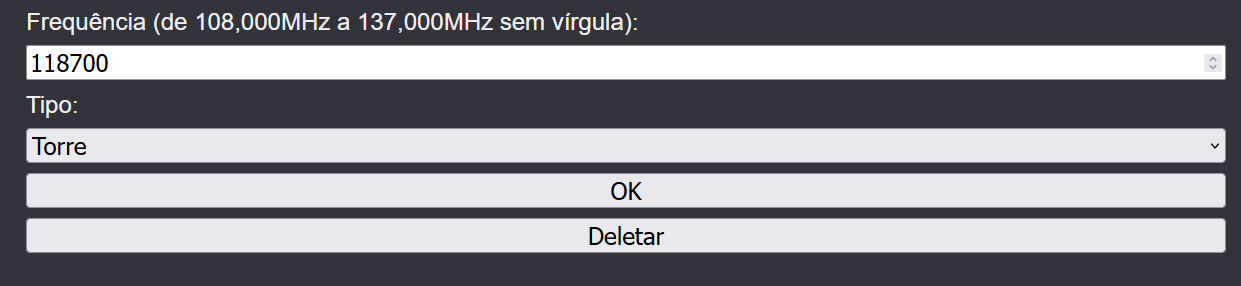
\includegraphics[width=0.7\linewidth]{img/admin-edit-comm.png}
    \caption{Tela de adicionar / editar uma frequência de comunicação}
    \label{fig:max-priv-sys}
    \end{center}
\end{figure}

As validações para esta rota são:
\begin{longtable}{|p{3cm}|p{4.5cm}|p{4.5cm}|}
    \caption{Editar comunicações} \\
    \hline
    \textbf{Campo} & \textbf{Frontend} & \textbf{Backend} \\ \hline
    \endfirsthead
    \multicolumn{3}{c}%
    {{\tablename\ \thetable{} -- Continuação da página anterior}} \\
    \hline
    \textbf{Campo} & \textbf{Frontend} & \textbf{Backend} \\ \hline
    \endhead
    \hline \multicolumn{3}{|r|}{{Continua na próxima página}} \\ \hline
    \endfoot
    \hline
    \endlastfoot
        Frequência
        & Deve ser de 108000 até 137000 (ambos inclusivos) (não deve ter vírgula. Por exemplo, a frequência 108,000MHz é digitada como 108000)
        & Deve ser de 108000 até 137000 (ambos inclusivos)
        \\ \hline
        Tipo
        & Menu dropdown (select/option)
        & Existe na lista de tipos de comunicações
        \\ \hline
\end{longtable}

\section {Adicionar/editar frequências de VOR}

São as frequências usadas para navegação, ao sintonizar
na frequência de uma antena VOR o avião pode voar diretamente para
ela. O nome de um localizador VOR é sempre formado por três letras
maíusculas.

\begin{figure}[H]
    \begin{center}
    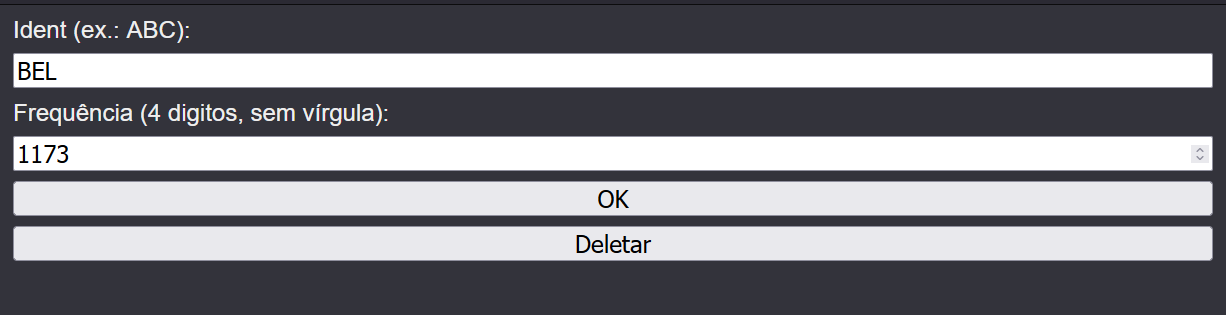
\includegraphics[width=0.7\linewidth]{img/admin-edit-vor.png}
    \caption{Tela de adicionar / editar um VOR}
    \label{fig:max-priv-sys}
    \end{center}
\end{figure}

As validações para esta rota são:
\begin{longtable}{|p{3cm}|p{4.2cm}|p{4.2cm}|}
    \caption{Adicionar/editar frequências de VOR} \\
    \hline
    \textbf{Campo} & \textbf{Frontend} & \textbf{Backend} \\ \hline
    \endfirsthead
    \multicolumn{3}{c}%
    {{\tablename\ \thetable{} -- Continuação da página anterior}} \\
    \hline
    \textbf{Campo} & \textbf{Frontend} & \textbf{Backend} \\ \hline
    \endhead
    \hline \multicolumn{3}{|r|}{{Continua na próxima página}} \\ \hline
    \endfoot
    \hline
    \endlastfoot
        Frequência
        & Deve ser de 1080 até 1180 (ambos inclusivos)
        & Deve ser de 1080 até 1180 (ambos inclusivos)
        \\ \hline
        Ident
        & \verb|^[A-Z]{3}$|
        & \verb|^[A-Z]{3}$|
        \\ \hline
\end{longtable}

\section {Adicionar/editar frequências de ILS}

\begin{figure}[H]
    \begin{center}
    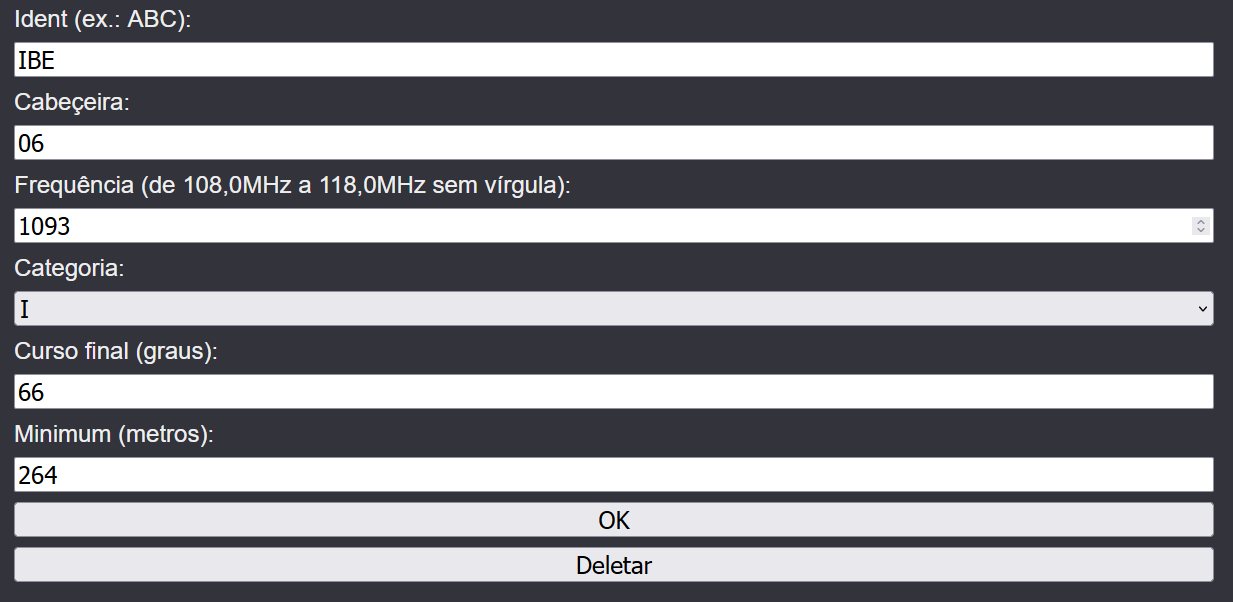
\includegraphics[width=0.7\linewidth]{img/admin-edit-ils.png}
    \caption{Tela de adicionar / editar um ILS}
    \label{fig:max-priv-sys}
    \end{center}
\end{figure}

As validações para esta rota são:
\begin{longtable}{|p{3cm}|p{4.2cm}|p{4.2cm}|}
    \caption{Adicionar/editar frequências de ILS} \\
    \hline
    \textbf{Campo} & \textbf{Frontend} & \textbf{Backend} \\ \hline
    \endfirsthead
    \multicolumn{3}{c}%
    {{\tablename\ \thetable{} -- Continuação da página anterior}} \\
    \hline
    \textbf{Campo} & \textbf{Frontend} & \textbf{Backend} \\ \hline
    \endhead
    \hline \multicolumn{3}{|r|}{{Continua na próxima página}} \\ \hline
    \endfoot
    \hline
    \endlastfoot
        Ident
        & Regex: \verb|^[A-Z]{3}$|
        & Regex: \verb|^[A-Z]{3}$|
        \\ \hline
        Cabeçeira
        & Regex: \verb|^\d{2}[LRC]?$|
        & Regex: \verb|^\d{2}[LRC]?$|
        \\ \hline
        Frequência
        & De 1080 até 1180 (ambos inclusive)
        & De 1080 até 1180 (ambos inclusive)
        \\ \hline
        Categoria
        & Menu dropdown (select/option)
        & Existe na lista de tipos de ILS
        \\ \hline
        Curso final
        & Type: Number
        & Inteiro
        \\ \hline
        Minimum
        & Type: Number
        & Inteiro
        \\ \hline
\end{longtable}


Um campo existente na tabela de aeródromo é o isPublished. Ele é usado para, no 
ato de criação, o aeródromo não aparecer vazio para o usuário final. Enquanto este 
campo está em false apenas usuários logados conseguem ver. Ao serem adicionadas 
as pistas, comunicações, VOR e ILS o botão de publicar pode ser pressionado fazendo 
esta variável ir para true, mostrando o aeródromo para todos que acessarem.
Quando um aeródromo é adicionado seu METAR e TAF não são atualizados automaticamente. 
É necessário que os trabalhos agendados pelo APS (Advanced Python Scheduler) 
atualizem estas informações. A função de atualização de gráficos (update\_images()) 
também é executada. Mesmo que, no início, exista apenas um METAR, o gráfico pode 
ser gerado sem problemas. Mas quando adiciono um aeródromo costumo esperar um 
tempo até publicá-lo, para termos vários METARs salvos deixando o gráfico com vários 
pontos no tempo.
